\chapter{Implementation}
\label{chap:implementation}
Bevor man mit dem Programmieren der Anwendung anfangen kann,
gilt es einiges vorzubereiten. Dieses Kapitel beschäftigt sich
mit der Microservice-Infrastruktur der Gesamtanwendung. Hier geht
es um das Aufsetzen einer agilen Infrastruktur, die den
stetigen Auslieferungsprozess der Software ermöglicht. 
In \Cref{chap:qualitaetssicherung} geht es um Methoden und Verfahren,
die die Qualität der Software sicherstellen. Erst nach der Erstellung
der Microservice-Infrastruktur sowie der Automatisierung von
Qualitätssicherungsprozessen, kann mit der Programmierung der
Anwendung begonnen werden.

Das Kapitel Microservice-Infrastruktur ist wie folgt gegliedert:
In \Cref{sec:continuousdelivery} befasst sich die Arbeit mit
dem stetigen Softwareauslieferungsprozess, bekannt als Continuous Delivery.
In \Cref{sec:monorepoundsubmodules} wird die Aufteilung der Versionsverwaltung
in einzelne Aufbewahrungsorte diskutiert. In \Cref{sec:infrastruktur}
wird die Infrastruktur der Gesamtanwendung geschildert. Hier geht es
um Technologien, die das Auslieferungsverfahren sowie die Benutzung
der Anwendung in Produktion ermöglichen. In \Cref{sec:systemdesign}
geht es um die Gestaltung der Anwendung selbst. Hier werden die einzelnen,
für die Anwendung nötigen Komponenten erörtert und definiert.
In \Cref{sec:pipelinedesign} geht es um die Pipeline, also den Auslieferungsprozess
selbst. Hier werden Vorkehrungen getroffen, um diesen zu ermöglichen.

\section{Continuous Delivery}
\label{sec:continuousdelivery}
Continuous Delivery (CD ist das Verfahren, Software in einem stetigen Zyklus auszuliefern.
Neue Technologien, wie die Containervirtualiserungssoftware Docker,
die im März 2013 von dotCloud ins Leben gerufen wurde \cite{DockerAbout2014}, vereinfachen
den stetigen Softwareauslieferungsprozess enorm. So kann man in einem automatisierten
Auslieferungsprozess, Images bauen, diese testen und selbige nach erfolgreichem
Bestehen der Tests in der Produktion verwenden. Eberhard Wolff schreibt über das Ziel von Docker in
seinem Buch "Continuous Delivery" folgendes: "Das Ziel von Docker ist es, Container für die
Distribution von Software zu nutzen. Im Vergleich zu normalen Prozessen trennen Linux-Container
einzelne Anwendungen viel besser voneinander, wenn es darum geht, die Software auf einem anderen
System zu installieren. Docker bietet ein Repository für Images an, so dass eine Vielzahl
von Servern mit identischen Images betrieben werden können."\cite[S. 56]{ContinuousDeliveryWolff}
Somit kann sichergestellt werden, dass die Software und deren Umgebung in der Testphase
sowie in Produktion die selbe ist. Immer mehr Anbieter stellen CI-Werkzeuge zur Verfügung,
die es ermöglichen eine CI/CD-Pipeline anhand von Konfigurationsdateien aufzuziehen. So bieten nun
neben Travis CI, CircleCI und Jenkins auch Versionsverwaltungshosts wie Github und
Gitlab CI-Werkzeuge zur Verfügung.\footnote{Github bietet seit 13. November 2019 eigene CI/CD-Werkzeuge an \cite{GithubCIToolsHeise}}
Vorteile eines CD-Ansatzes sind schnelle Feature-Auslieferung und somit schnellere Resonanz der Benutzer auf die Features,
Robustheit der Software durch stetiges Ausführen automatisierter Tests in der Pipeline, einfaches Zurückrollen
der Version der Anwendung in Produktion sowie einfaches Reproduzieren von Fehlern. Ein Nachteil eines CI/CD-Ansatzes ist
der große Aufwand des initialen Aufbaus der automatisierten Prozesse. Bei komplexen Änderungen des Systems müssen zudem
große Teile des automatisierten Prozesses angepasst werden.

In der Arbeit wird für die Versionsverwaltung und die stetige Softwareauslieferung ein eigener Linux-Server verwendet,
auf dem die Community Version von Gitlab installiert ist. Auf dem Linux-Server befinden sich auch eine eigene Docker
Registry sowie ein eigener Gitlab Runner\footnote{Gitlab Runner dienen zur Ausführung der Pipeline}. Der Aufbau
wird in \Cref{sec:infrastruktur} nochmal genauer behandelt. 

\section{Monorepo und Submodules}
\label{sec:monorepoundsubmodules}
In diesem Abschnitt geht es um die Aufteilung des Programmcodes in Repositories. Für die Versionsverwaltung
wird Git verwendet. Die Arbeit entscheidet sich dazu, die einzelnen Microservices in einer Monorepo unterzubringen.
Unter Monorepo versteht man die Strategie, den Programmcode aus mehreren Anwendungen, Services, Bibliotheken und Frameworks
in einer Repository unterzubringen.\cite{MonorepoTrunkBasedDevelopment} Diese Strategie verringert nicht nur den Aufwand
des Aufsetzens mehrerer Repositories, sondern gibt den Entwicklern auch einen besseren Überblick über die einzelnen
Projekte. Gerade im Fall von Microservices hat dieser Ansatz den Vorteil, dass man Änderungen in mehreren Services,
die miteinander verkoppelt sind, in einem Commit in die Versionsverwaltung einchecken kann. Dies kann verbindlich sein,
wenn Tests der Pipeline auf bestimmte Versionen der unterschiedlichen Services angewiesen sind. Verändert man beispielsweise
eine API eines Services, kann man gleichzeitig das Frontend anpassen. Die Diagramme eines Dashboards sollen allerdings
auch extern entwickelbar sein. Um dies zu ermöglichen, verwendet die Arbeit Git-Submodules.\cite{GitsubmodulesGitSCM} Mithilfe dieser Submodules
kann man andere Repositories in ein Repository integrieren. Somit können externe Entwickler das Repository des
Submodules gabeln\footnote{Unter "gabeln" oder auch "forken" versteht man das Erstellen einer eigenen Kopie eines Repositories, mit der unabhängig von der Versionierung der gegabelten Repository entwickelt werden kann.},
um in ihrem eigenen Repository Diagramme für die Anwendung zu entwickeln.

\section{Infrastruktur}
\label{sec:infrastruktur}
Wie in \Cref{sec:continuousdelivery} bereits angesprochen, beinhaltet die Infrastruktur
der Arbeit einen Linux-Server, auf welchem Gitlab CE, Gitlab Runner und eine Docker Registry
installiert sind. Desweiteren benötigt es weitere Server, für die Testphase sowie für
die Produktion. Die einzelnen Services werden einfachheitshalber mithilfe von Docker-Compose
auf einem einzelnen Server ausgeführt. Das Ziel für die Zukunft ist es, die einzelnen
Services auf einzelne Linux-Server zu verteilen. Dies soll mithilfe des Open Source IAC-Werkzeugs\footnote{IAC steht für Infrastructure as Code}
Terraform über eine Cloudanbieter-API und dem Orchestrierungssystem Kubernetes automatisiert werden.
Die Arbeit beschränkt sich allerdings auf drei Linux-Server. Einen für die Versionsverwaltung
und den CI/CD-Prozess, einen für die Testphase sowie einen für die Produktion. 
Die drei Server werden von Hetzner, einem Cloudanbieter, bereitgestellt und haben Ubuntu 18.04
vorinstalliert.\footnote{Die 3 Linuxserver haben 4 VCPUs, 16GB RAM und 160GB SSD-Speicher} 
Neben den Servern benötigt es noch Volumes, um die Daten der Datenbanken zu persistieren.
Die an die Server angebrachten Volumes werden mithilfe von Docker-Compose auf die für die
Beständigkeit relevanten Ordner der Datenbank-Container zugewiesen. Die Zuweisung variiert
je nach Datenbank. Um die Server über das Internet zu erreichen, benötigt es diverse Domains
und Subdomains, die mithilfe von DNS-Records auf die vom Server bereitgestellten
IPv4- und IPv6-Adressen verweisen.\footnote{Man kann die Server natürlich auch direkt über die IP-Adresse ansprechen.}

Die Domain "blicc.org" dient als Hauptdomain und wird in der Produktion verwendet. Der Name Blicc
wurde zur representation des Produktes gewählt. Bei einer Verwendung der Anwendung als White-Label-Produkt
wird der Name durch den der zu repräsentierenden Firma ersetzt. Der Name Blicc ist eine
veränderte Form des deutschen Wortes "Blick". Der Name wurde daher verändert, da die Verfügbarkeit
von "Blick" in den meisten Domainvariationen nicht mehr erhältlich war und zudem
überteuert angeboten wurde. Die Domain für den Server der Testphase ist "testing-stage.org".
Die beiden Domains besitzten die Subdomains "api" und "delivery". Die Subdomain "api" verweist
auf die Resource Management API; die Subdomain "delivery" verweist auf die Data Delivery API.
Desweiteren gibt es die "monitor" Subdomain, welche auf die Kontrollübersicht von Traefik
verweist. Traefik dient als Reverse-Proxy und Load-Balancer, bietet zusätzlich allerdings
auch noch geringe Überwachungsfunktionalitäten in einem webbasierten Dashboard an.
Dazu mehr in \Cref{subsec:reverseproxyundloadbalancer}.

Die Docker Registry ist unter der Domain "registry.thiloilg.com", Gitlab CE
unter "gitlab.thiloilg.com" erreichbar. Die Repositories werden alle zusätzlich
auf Github.com gespiegelt. Github.com dient als drittes Backup, falls die Repositories auf dem
eigenen Gitlab Server und dem lokale Rechner verloren gehen. Mit dem Git-Befehl in
Quellcode \ref{lst:gitalias} kann man sich einen Alias setzen, um zu allen Remote Repositories
gleichzeitig zu pushen. Der senkrechte Strich im Linux Terminal, bekannt als "Pipe", trennt zwei Befehle in der
Kommandozeile. Das Ergebnis des ersten Befehls wird an den zweiten Befehl weitergereicht.

\begin{listing}
    \inputminted{sh}{snippets/sh/pushall.sh}
    \caption{Konfiguration eines eigenen Git Alias}
    \label{lst:gitalias}
\end{listing}

Für das Aufsetzen der Server benötigt man drei Schritte.
Als erstes verbindet man sich über SSH zu dem Server und richtet den die UFW
ein.\footnote{UFW steht für Uncomplicated Firewall} Dabei öffnet man alle Ports,
die von den Anwendungen des Server benötigt werden. In der Regel sind das Port 80
für HTTP und Port 443 für HTTPS. Aufgrunddessen, dass bei dem Gitlab CE Server
Port 22 bereits für die SSH verbindung benötigt wird, musste der Gitlab Shell SSH
Port auf 2222 verlegt werden. Als zweiten Schritt Installiert man alle nötigen
Programme auf dem Server. Das wichtigste der Programme ist Docker CE. In Schritt
drei kopiert man mithilfe von SCP die \code{docker-compose.yml} Datei auf den
Server und startet sie mit \code{docker-compose up}. In der Docker-Compose Datei
stehen alle wichtigen Informationen, um ein kleines Docker-Cluster aufzuziehen.
Bei dem Server für die Testphase sowie dem Produktionsserver ist dieser Prozess
in der Gitlab CI Pipeline automatisiert. Eine genauere Beschreibung der
Pipeline befindet sich in \Cref{sec:pipelinedesign}.

\section{Systemdesign}
\label{sec:systemdesign}
In diesem Abschnitt wird das Grundkonzept aus \Cref{subsec:trennungvonlogic}
über die Trennung von Logik weiter ausgebaut und daraus ein komplettes System
entwickelt. Komponentenspezifische Implementierungsdetails
werden in \Cref{chap:komponentendesign} vorgestellt. 
Dieser Abschnitt fokussiert sich auf die Merkmale der Komponenten,
die für das Gesamtsystem von relevanz sind. In \Cref{subsec:systemuebersicht} verschafft
sich die Arbeit einen groben Überblick über das System. Anhand einer Grafik wird das Zusammenspiel
der einzelnen Komponenten erläutert. In  \Cref{subsec:reverseproxyundloadbalancer}
wird der Reverse Proxy und der Load Balancer behandelt.
Dabei stellen sich folgende Fragen: Wie muss die Schnittstelle der
Infrastruktur zur Außenwelt aussehen? Was muss man einhalten, um späteres
Skalieren zu ermöglichen? In \Cref{subsec:inhaltsauslieferung} wird
die Inhaltsauslieferung vorgestellt. Dabei stellt sich die Frage,
wie die Ressourcen möglichst performant an die Clients transportiert
werden können. In \Cref{subsec:wahlderdatenbankarten} geht es um die Wahl
der Datenbankart der einzelnen Services. Abschließend setzt sich die Arbeit
in \Cref{subsec:ueberwachungundwartung} mit der Überwachung und Wartung
des Systems auseinander.

\subsection{Systemübersicht}
\label{subsec:systemuebersicht}
Die Abbildung \ref{figure:uebersichtueberdassystemdesign} verschafft einen guten Überblick
über das Zusammenspiel der einzelnen Komponenten. Im oberen Bereich sieht man die
Frontendanwendung sowie eine Repräsentation einer externen API. Die Frontendanwendung
besteht aus dem Frontend sowie dem integrierten Plugin-System. Je nach Kommunikationsart
unterhält sich das Frontend über HTTPS oder WSS mit dem Backend. Die HTTPS-Kommunikation
wird durch einen Service Worker interferiert, um das Frontend-Caching und die
Offline-Funktionalität zu ermöglichen. Das WebSocket-Protokoll verbindet das Frontend
über direktem Web mit dem Backend. Dies kann allerdings von Browser zu Browser variieren.
Mache Versionen der Browser enthüllen die WebSocket-Kommunikation im SW, andere
nicht.\footnote{Siehe Diskussion auf Github, W3C Service Worker\cite{GithubIssueWebSocketExpose}}
Die Kommunikation zwischen externen APIs und dem Backend kann über HTTP als auch
HTTPS erfolgen. Zukünftige Kommunikationen über WebSockets oder QUIC\footnote{QUIC (Quick UDP Internet Connections) ist ein von Google entwickeltes, auf UDP basierendes Transportprotokoll.\cite{IETFQUICWhatsHappening} Die IETF arbeitet an einer Standardisierung des Internetprotokolls.\cite{DatatrakcerIETFQuic}}
sind denkbar.

\begin{figure}
    \begin{center}
    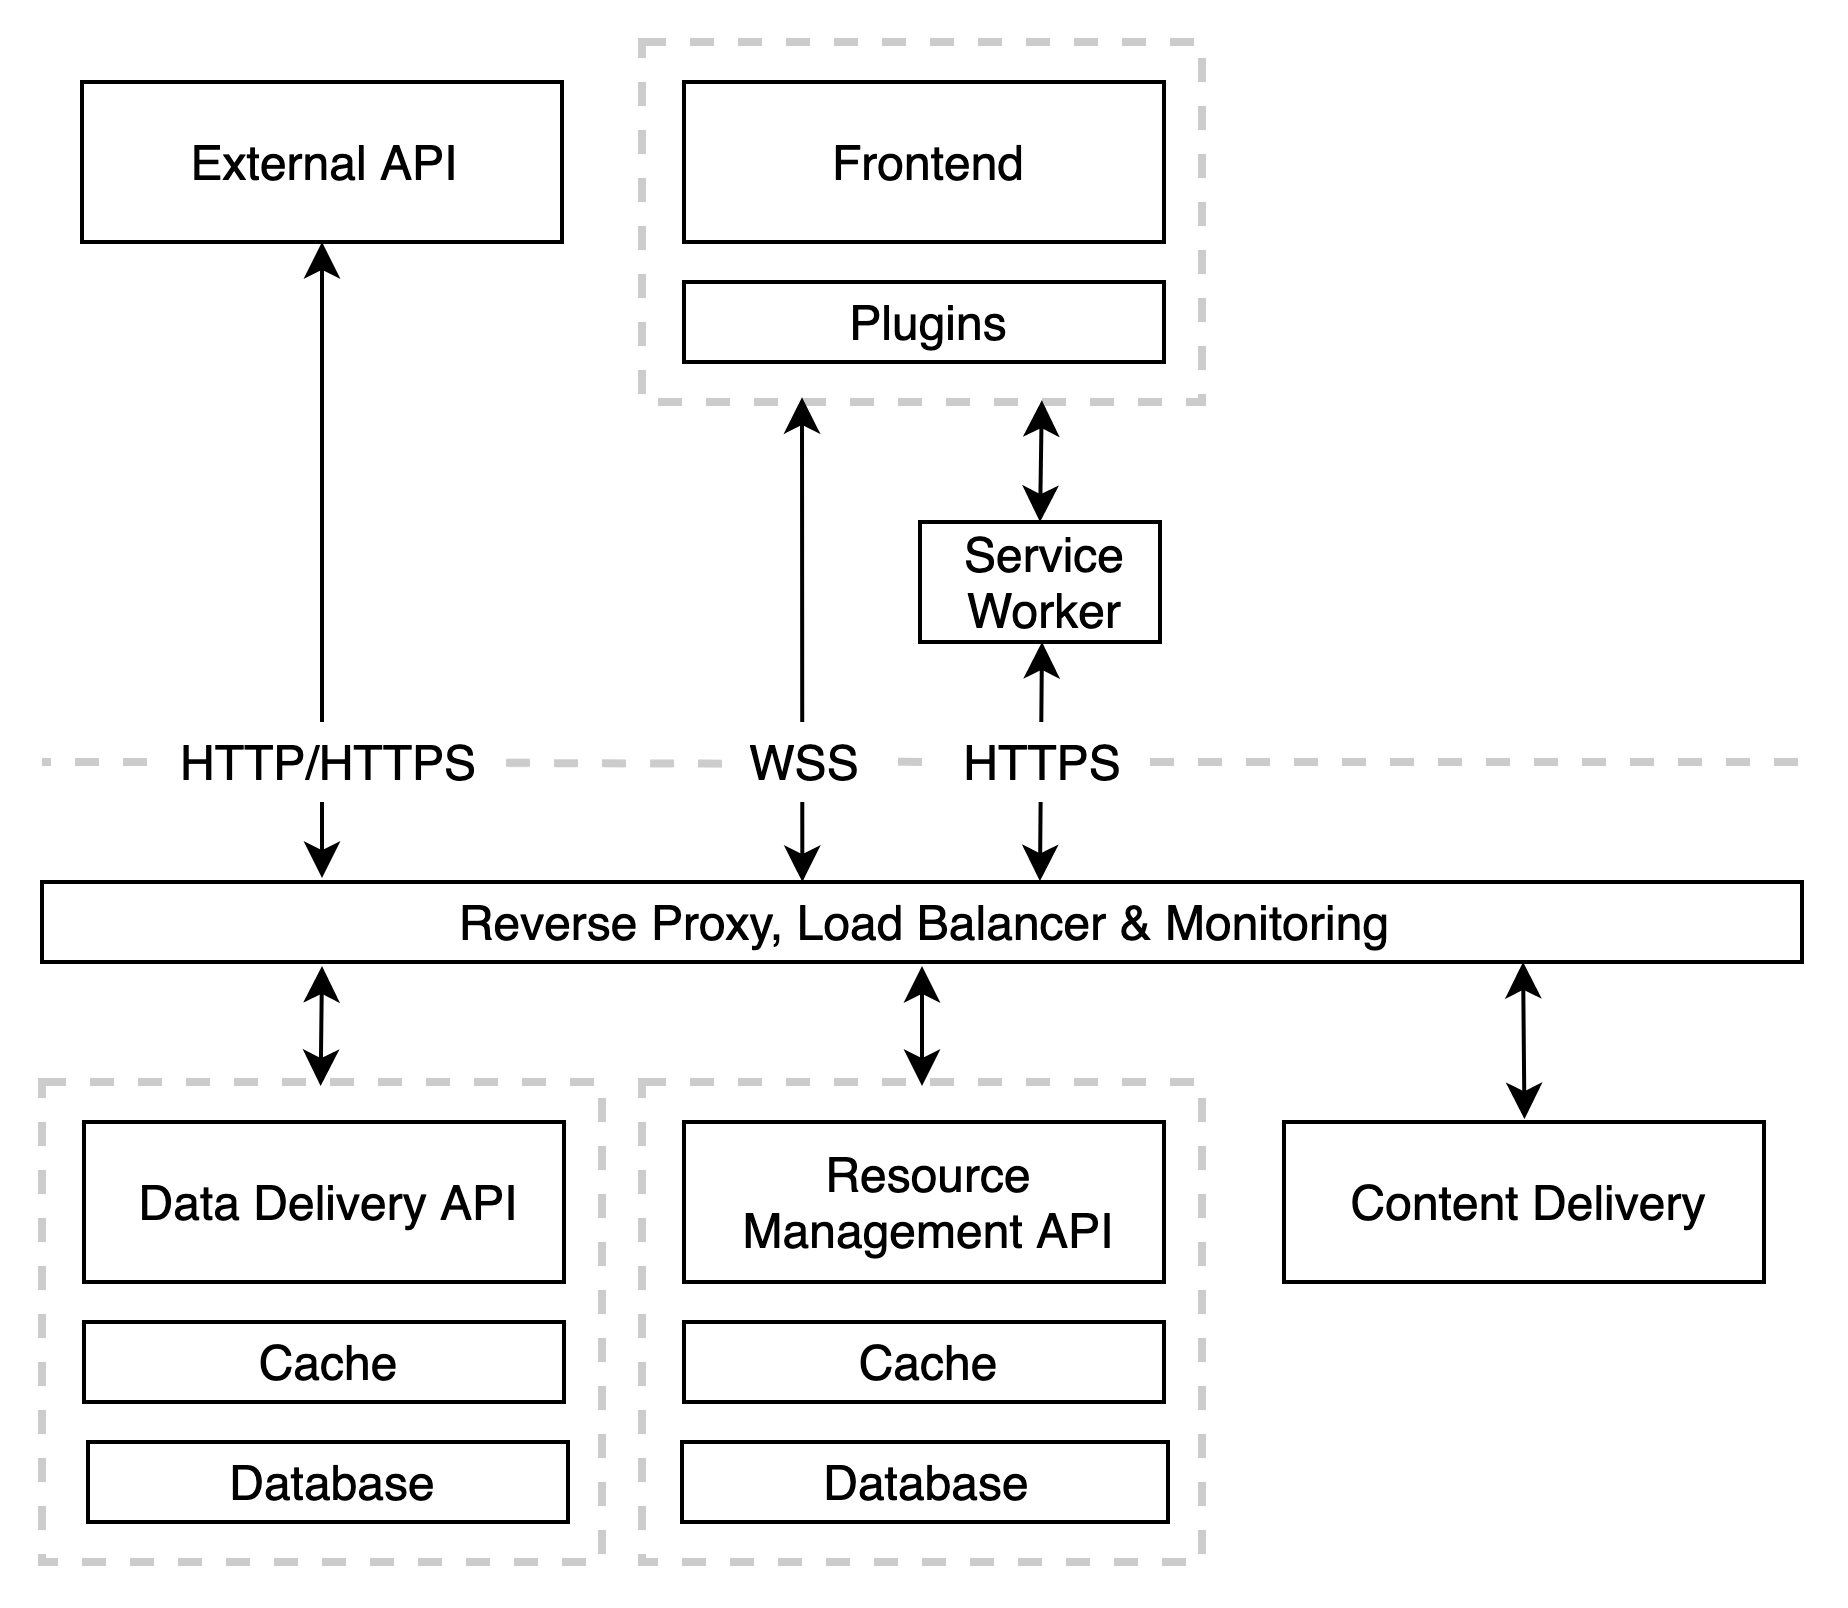
\includegraphics[scale=0.2]{img/abbildungen/MicroserviceInfrastruktur}
    \end{center}
    \caption{Übersicht über das System}
    \label{figure:uebersichtueberdassystem}
\end{figure}

Das Backend und dessen Microservice-Infrastruktur wird durch einen Reverse Proxy vom Internet versteckt.
In dieser Zwischenschicht befinden sich unter anderem ein Load Balancer sowie ein Monitoring System.
Das Backend ist in drei Services unterteilt; die Data Delivery API, die Resource Management API
und den Content Delivery Service. Die Data Delivery API sowie die Resource Management API sind jeweils
in drei Container unterteilt. Der wichtigste Container führt die Servicelogik aus. In der zweiten
Schicht befindet sich eine In-Memory-Datenbank, die für das Caching verantwortlich ist. Zuallerletzt
kommt eine Datenbank, um den Fortbestand der Daten zu sichern. Die Caching-Strategie sowie die Art der
Datenbank variiert je nach Anforderung an den Service. Für die Langzeitspeicherung der Daten wird je nach Service
eine dokumentenorientiertes als auch ein relationales Datenbanksystem verwendet. Der Content Delivery Service
ist für die Auslieferung der statischen Dateien des Frontends verantwortlich. Hier ist die Wahl des
richtigen Kompressionsverfahrens ausschlaggebend.

\subsection{Reverse Proxy und Load Balancer}
\label{subsec:reverseproxyundloadbalancer}
Anders, als bei einem Proxy, der den Client von dem Server versteckt, versteckt ein Reverse Proxy
eine Serverinfrastruktur vor dem Client. Durch die Anonymisierung der Serverinfrastruktur
sind Angriffe gegen spezifische Servertechnologien erschwert, da deren Schnittstelle
nicht direkt mit der Außenwelt kommuniziert. In der Regel übernimmt der Reverse Proxy
auch die SSL/TLS-Verschlüsselung. Desweiteren kann er auch zur Verteilung der Serverlast,
also als Load Balancer verwendet werden. Ein typisches Beispiel für einen Reverse Proxy
ist ein Nginx Webserver. Die Arbeit benutzt als Reverse Proxy und Load Balancer die
in Golang geschriebene Open Source Software Traefik.\footnote{https://docs.traefik.io/}
Traefik unterstützt die Kommunikation mit Orchestrierungssystemen wie Kubernetes
und Docker Swarm, und bietet additional auch noch automatisierte SSL/TLS-Verschlüsselung
mithilfe von Let's Encrypt.\footnote{https://letsencrypt.org/} Laut einer Google Checklist,
ist eine Verbindung über HTTPS Vorraussetzung für eine PWA.\cite{GooglePWAChecklist}
Ohne SSL/TLS-Verschlüsselung werden Funktionalitäten wie das hinzufügen der App zum Homescreen
von den Browsern nicht bereitgestellt. Verschlüsselungsschichten wie TLS und der Vorgänger
SSL liegen zwischen der TCP-Schicht und HTTP/WS. Neben dem Public-Key-Verschlüsselungsverfahren
muss für eine TLS-Verschlüsselung auch die Authentizität des Servers, mit dem kommuniziert wird,
bestätigt sein. Hierfür benötigt man ein EV-TLS-Zertifikate\footnote{EV steht für Extended Validation}
Mithilfe von Let's Encrypt, einer gemeinnützigen Zertifizierungsstelle, kann man EV-TLS-Zertifikate
kostenlos über eine API beantragen. Die Arbeit hat sich unter anderem für Traefik entschieden,
da der Reverse Proxy einen automatisierten Vorgang bereitstellt, indem EV-TLS-Zertifikate
mithilfe von Let's Encrypt generiert werden.

Ein Load Balancer entscheidet, wie die Serverlast unter den verschiedenen Services aufgeteilt wird.
Das einfachste Lastverteilungsverfahren ist ein Round-Robin DNS, eine rotierende Verteilung
der eingehenden Anfragen auf unterschiedliche IP-Adressen.\cite{CloudflareRoundRobinDNS} 
Da die Aufrechterhaltung der WebSocket-Verbindungen der Data Delivery API gegenüber
den Clients allerdings nicht linear verlaufen wird,\footnote{Manche Benutzer beenden die Anwendung sofort, andere lassen Sie über Tage laufen.}
empfiehlt sich hier die Implementierung einer anhand von Health-Checks basierenden
Lastverteilungsverfahren. Man schaut in überschaubaren Abständen nach der aktuellen
Lastverteilung und weißt die Anfragen so dem am wenigsten überlasteten Service zu.
Die Arbeit konzentriert sich hier auf die Ermöglichung eines solchen Verfahrens,
indem die Schicht der Servicelogik zustandslos gestaltet wird. Somit ist eine
horizontale Skalierung der Serviceinstanzen problemlos möglich. Mehr dazu in
\Cref{subsec:authentifizierungsverfahren}.

\subsection{Inhaltsauslieferung}
\label{subsec:inhaltsauslieferung}
Die Inhaltsauslieferung ist dafür zuständig, statische Inhalte der Frontendanwendung
an den Client auszuliefern. Die statischen Inhalte sind unter anderem
HTML-, CSS- und JS-Dateien, JSON-Dateien wie das Web App Manifest sowie Bilddateien.
Hierfür ist es üblich, einen Webserver wie Nginx zu verwenden. Steve Souders betont
in einem Vortrag über die Performance von JavaScript, dass ein Drittel der im Browser
geladenen First-Party-Scripts zwischen 90- und 100Kb nicht komprimiert werden.
Das liege daran, dass jQuery, eine der meistgenutztesten JS-Bibliotheken,
unkomprimiert circa bei 100Kb angesiedelt sei.\cite{SteveSoudersMakeJavaScriptFaster}
Laut einer Statistik von Build With benutzten 88,07\% der Top 10k meinstbesuchtesten
Webseiten des Internets jQuery.\footnote{Stand Februar 2020}\cite{BuildWithjQuery}

Um die Relevanz der Kompression von Daten zu verdeutlichen, führt diese Arbeit einen
Vergleichstest des initialen Ladevorgangs der Frontendanwendung,
einmal mit Gzip, Brotli und einmal ohne Kompression durch. Brotli ist eine
von Zoltán Szabadka und Jyrki Alakuijala entwickeltes Kompressionsverfahren,
dass auf die Entropiekodierung Huffman und dem verlustlosen
Datenkompressionsverfahren LZ77 basiert.\cite{BrotliGoogleOpenSourceBlog}
Die unkomprimierte Größe der Frontendanwendung beträgt 819KB. Die Leistungstests
werden mit dem Open-Source-Werkzeug Lighthouse durchgeführt.\footnote{https://developers.google.com/web/tools/lighthouse}
Um den Unterschied der benötigten Zeit zum initialen Laden der Frontendanwendung
besser zu verdeutlichen, wird der Datendurchlauf auf 1.638,4Kbps verringert.
Die Frontendanwendung wird in einem nachgeahmten Nexus 5X ausgeführt.
Für die Analyse wurden vier Metriken aus dem Testbericht entnommen.
Die Ergebnisse des Leistungstests sind in Abbildung \ref{tab:lighthouseleistungstestdesinitialenladevorgangs}
dargestellt.

\begin{table}[h]
    \begin{center}
\begin{tabular}{l*{8}{r}}
Metrik & Ohne Kompr. & Gzip & Brotli \\
\hline
Erstes Zeichnen von Inhalten & 6,2s  & 3,1s & 2,9s \\
Erste CPU-Inaktivität        & 6,2s  & 4,3s & 4,1s \\
Zeit für Interaktion         & 7,5s  & 4,3s & 4,1s \\
Übertragungsgröße            & 1.172KB  &  553KB & 481KB \\
\end{tabular}
\end{center}
\caption{Lighthouse Leistungstest des initialen Ladevorgangs}
\label{tab:lighthouseleistungstestdesinitialenladevorgangs}
\end{table}

Die Zeit wird von der ersten vom Browser ausgehenden Anfrage gemessen.
Lighthouse beschreibt die Metriken wie folgt: Unter dem ersten Zeichnen
von Inhalten versteht man den ersten Zeitpunkt, an dem der Browser
irgendeinen Inhalt zeichnet. Die erste CPU-Inaktivität ist
der erste Zeitpunkt, an dem die Seite auf Benutzerinteraktionen reagieren könnte.
Unter Zeit für Interaktion versteht man den Zeitpunkt, an dem alle Inhalte geladen ist.
Jetzt kann die Seite zu jeder Interaktion schnell reagieren.\cite{WhatPerformanceMetricsMeasure}

In Abbildung \ref{tab:lighthouseleistungstestdesinitialenladevorgangs} wird klar deutlich,
dass Kompression gerade bei langsameren Internetverbindungen von großer Bedeutung ist.
Es ist wichtig anzumerken, dass der Brotli-Kompressionsalgorithmus zwar eine größere
Kompressionsrate besitzt, allerdings für die Kompression und Dekompression mehr Zeit
benötigt.\cite{CompressionBenchmark} Für dynamische Inhalte sollte man also Gzip
benutzen. Wichtig ist auch, dass Bilder je nach Format in der Regel bereits komprimiert wurden.
Ein weiterer Kompressionsvorgang kann die Größe der Bilder vergrößern.

Die Arbeit verwendet wie bereits erwähnt einen Nginx Webserver für die
Auslieferung von statischen Inhalten. Für die Zukunft sollte man die Nutzung
eines CDNs in Betracht ziehen, um die weltweite Ladezeit zu optimieren.

\subsection{Wahl der Datenbankarten}
\label{subsec:wahlderdatenbankarten}
Die Data Delivery API verwendet ein dokumentenorientiertes Datenbanksystem.
Hauptgrund hierfür ist die Tatsache, dass man nicht im Vorhinein weiß, wie das
Datenschema auszusehen hat. Der Benutzer der Anwendung kann jegliche API
auswählen, Daten abfragen und diese mithilfe einer JSON-Abfragesprache verarbeiten. Das Datenschema
kann sich also während der Laufzeit des Programms verändern. Im Gegensatz hierzu steht die Resource
Management API, welche auf eine relationale Datenstruktur aufgebaut ist. Die Schemata formen das
Erscheinungsbild der API und werden als CRUD-Operationen über eine REST-Schnittstelle enthüllt.
Nun stellt sich aber die Frage, wieso man für die Resource Management API nicht auch eine
No-SQL-Datenbank verwendet hat. Clemens Gull bringt die Kompromisse, welche man bei der
Entscheidung zwischen einem relationalen und einem dokumentenorientierten DBMS
eingehen muss, in seinem Buch "Wev-Applikationen entwickeln mit NoSQL" auf den Punkt:
"Da RDBMS (relationale Datenbankmanagementsysteme, also konventionelle Datenbanken) sehr streng
auf die Konsistenz der Daten achten, kann es hier zu Problemen mit der Performance und Verfügbarkeit
kommen. Dieses Konzept wird bei NoSQL zugunsten der besseren Skalierbarkeit und auch Verfügbarkeit
aufgeweicht."\cite[S. 18]{NoSQLClemensGull} Um die bessere Verfügbarkeit bei dokumentenorientierten
DBMS zu garantieren, wird bewusst auf die Normalisierung
\footnote{Frank Geisler zur Normalisierung: "Die Normalisierung reduziert die in der Datenbank vorhandenen Datenredundanzen und hilft Ihnen so dabei, die \dots Anomalien zu vermeiden."\cite[S. 177]{DatenbankenFrankGeisler}}
verzichtet. Durch die dadurch entstehende Redundanz in der Datenbank fällt es schwer,
die Konsistenz der Daten zu garantieren. Desweiteren ist der Schreibvorgang bei dokumentenorientierten
DBMS wie MongoDB nur auf Dokumentenebene atomar.\cite{MongoDBAtomaritaet} Da die Konsistenz und Atomarität für
Benutzerverwaltungsdaten von erheblicher relevant ist\footnote{Speziell bei sensiblen Transaktionen wie Zahlungsabläufen.}, 
entscheidet sich die Arbeit für die Resource Management API ein RDBMS zu verwenden.
Um das Performanzdefizit im vergleich zu dokumentbasierenden DBMS auszugleichen,
werden Indices verwendet. Ein Datenbankindex ist ein Kompromiss, bei dem
man Speicherplatz gegen Zugriffsgeschwindigkeit tauscht.\cite{YoutubePostgresIndexing}
Mithilfe einer aktuell gehaltenen Indexstruktur\footnote{Beispielsweise Binärbäume, Hashtabellen und sortierte Abfolgen}
wird die Komplexität eines Spaltenzugriffs dezimiert.

\subsection{Überwachung und Wartung}
\label{subsec:ueberwachungundwartung}
Essentiell für die Überwachung der Services ist eine solide Protokollierung.
Die Arbeit beschränkt sich hier auf drei Protokollebenen; Error, Info und Debug.
Error ist die tiefste Ebene. Hier werden die während der Laufzeit des Programms
stattgefundenen Fehler protokolliert. Auf der Info-Protokollebene sieht man
aufschlussreiche Informationen über den Service. Hier wird beispielsweise
der HTTP-Verkehr aufgezeichnet. Die Error-Protokollebene ist in der Info-Protokollebene
enthalten. In der Debug-Ebene erscheinen die beiden zuvor erwähnten Ebenen. Diese
werden mit Informationen angereichert, die nur für das Debugging relevant sind.
Ein Logeintrag besteht aus einem Zeitstempel, der Protokollebene sowie der Protokollnachricht.
Kundenspezifische Informationen werden nicht offengelegt. Verweise auf Nutzer finden nur
mithilfe der Identifikationsnummer des Datenbankeintrags statt. Die Info-Protokollebene
wird über den \code{stdout} gelenkt. Die Error-Protokollebene wird desweiteren in einer
Logdatei persistiert. Für das Debugging muss die Debug-Protokollebene aktiviert werden.
Als Logging-Bibliothek für die Resource Management API verwendet die Arbeit den Winston
Logger. Der HTTP-Verkehr wird mithilfe des Koa-Loggers\footnote{Koa ist ein HTTP Middleware Framework für Node.js} protokolliert und an den Winston
Logger weitergereicht. Datenbankverbinder sowie Logger werden mithilfe des Singleton-Pattern
implementiert, um das ständige herunterreichen von Instanzen zu vermeiden. Der komfortabelste
Weg in JavaScript ein Singleton zu erstellen, ist, indem man ein Objekt exportiert. JavaScript-Objekte
werden beim initialen Ladevorgang in den Cache gesetzt. JavaScript sorgt dafür,
dass bei allen weiteren Zugriffen auf das Objekt, die selbe Instanz zurückgegeben wird.\cite{NodeJsCaching}

Der Reverse Proxy Traefik stellt eine Übersicht über die im HTTP-Verkehr gesendeten 
HTTP-Statuscodes. Die einzelnen Services besitzen Health-Checks, die den aktuellen
Gesundheitsstatus der Serviceinstanz widerspiegeln. Um die Wartung der Services zu erleichtern,
werden bei jedem Pipeline-Durchlauf unbenutzte Container, Netzwerke und Images
entfernt sowie der Cache entleert.

\section{Pipeline Design}
\label{sec:pipelinedesign}
Um eine stetige Softwareauslieferung zu ermöglichen, benötigt es einen automatisierten
Prozess. Dieser Prozess muss sich um das Bauen, Testen und Ausliefern der einzelnen
Container kümmern. In Abbildung \ref{figure:uebersichtueberdenstetigenauslieferungsprozess}
sieht man eine Übersicht über den Auslieferungsprozess. An der X-Achse entlang sieht
man die unterschiedlichen Umgebungen. Als erstes ist dort die Pipeline, ein in einem
Gitlab Runner ausgelagerter Prozess, der ein vordefiniertes Script durchläuft.
Damit der Gitlab Runner weiß, was er zu tun hat, werden in der \code{.gitlab-ci.yml}
Datei einzelne Abschnitte und deren Aufgaben mithilfe der vereinfachten
Auszeichnungssprache YAML definiert. Für jeden Abschnitt kann ein eigenes Docker-Image
gewählt werden. Mehr dazu findet man in \Cref{subsec:stages}.

\begin{figure}
    \begin{center}
    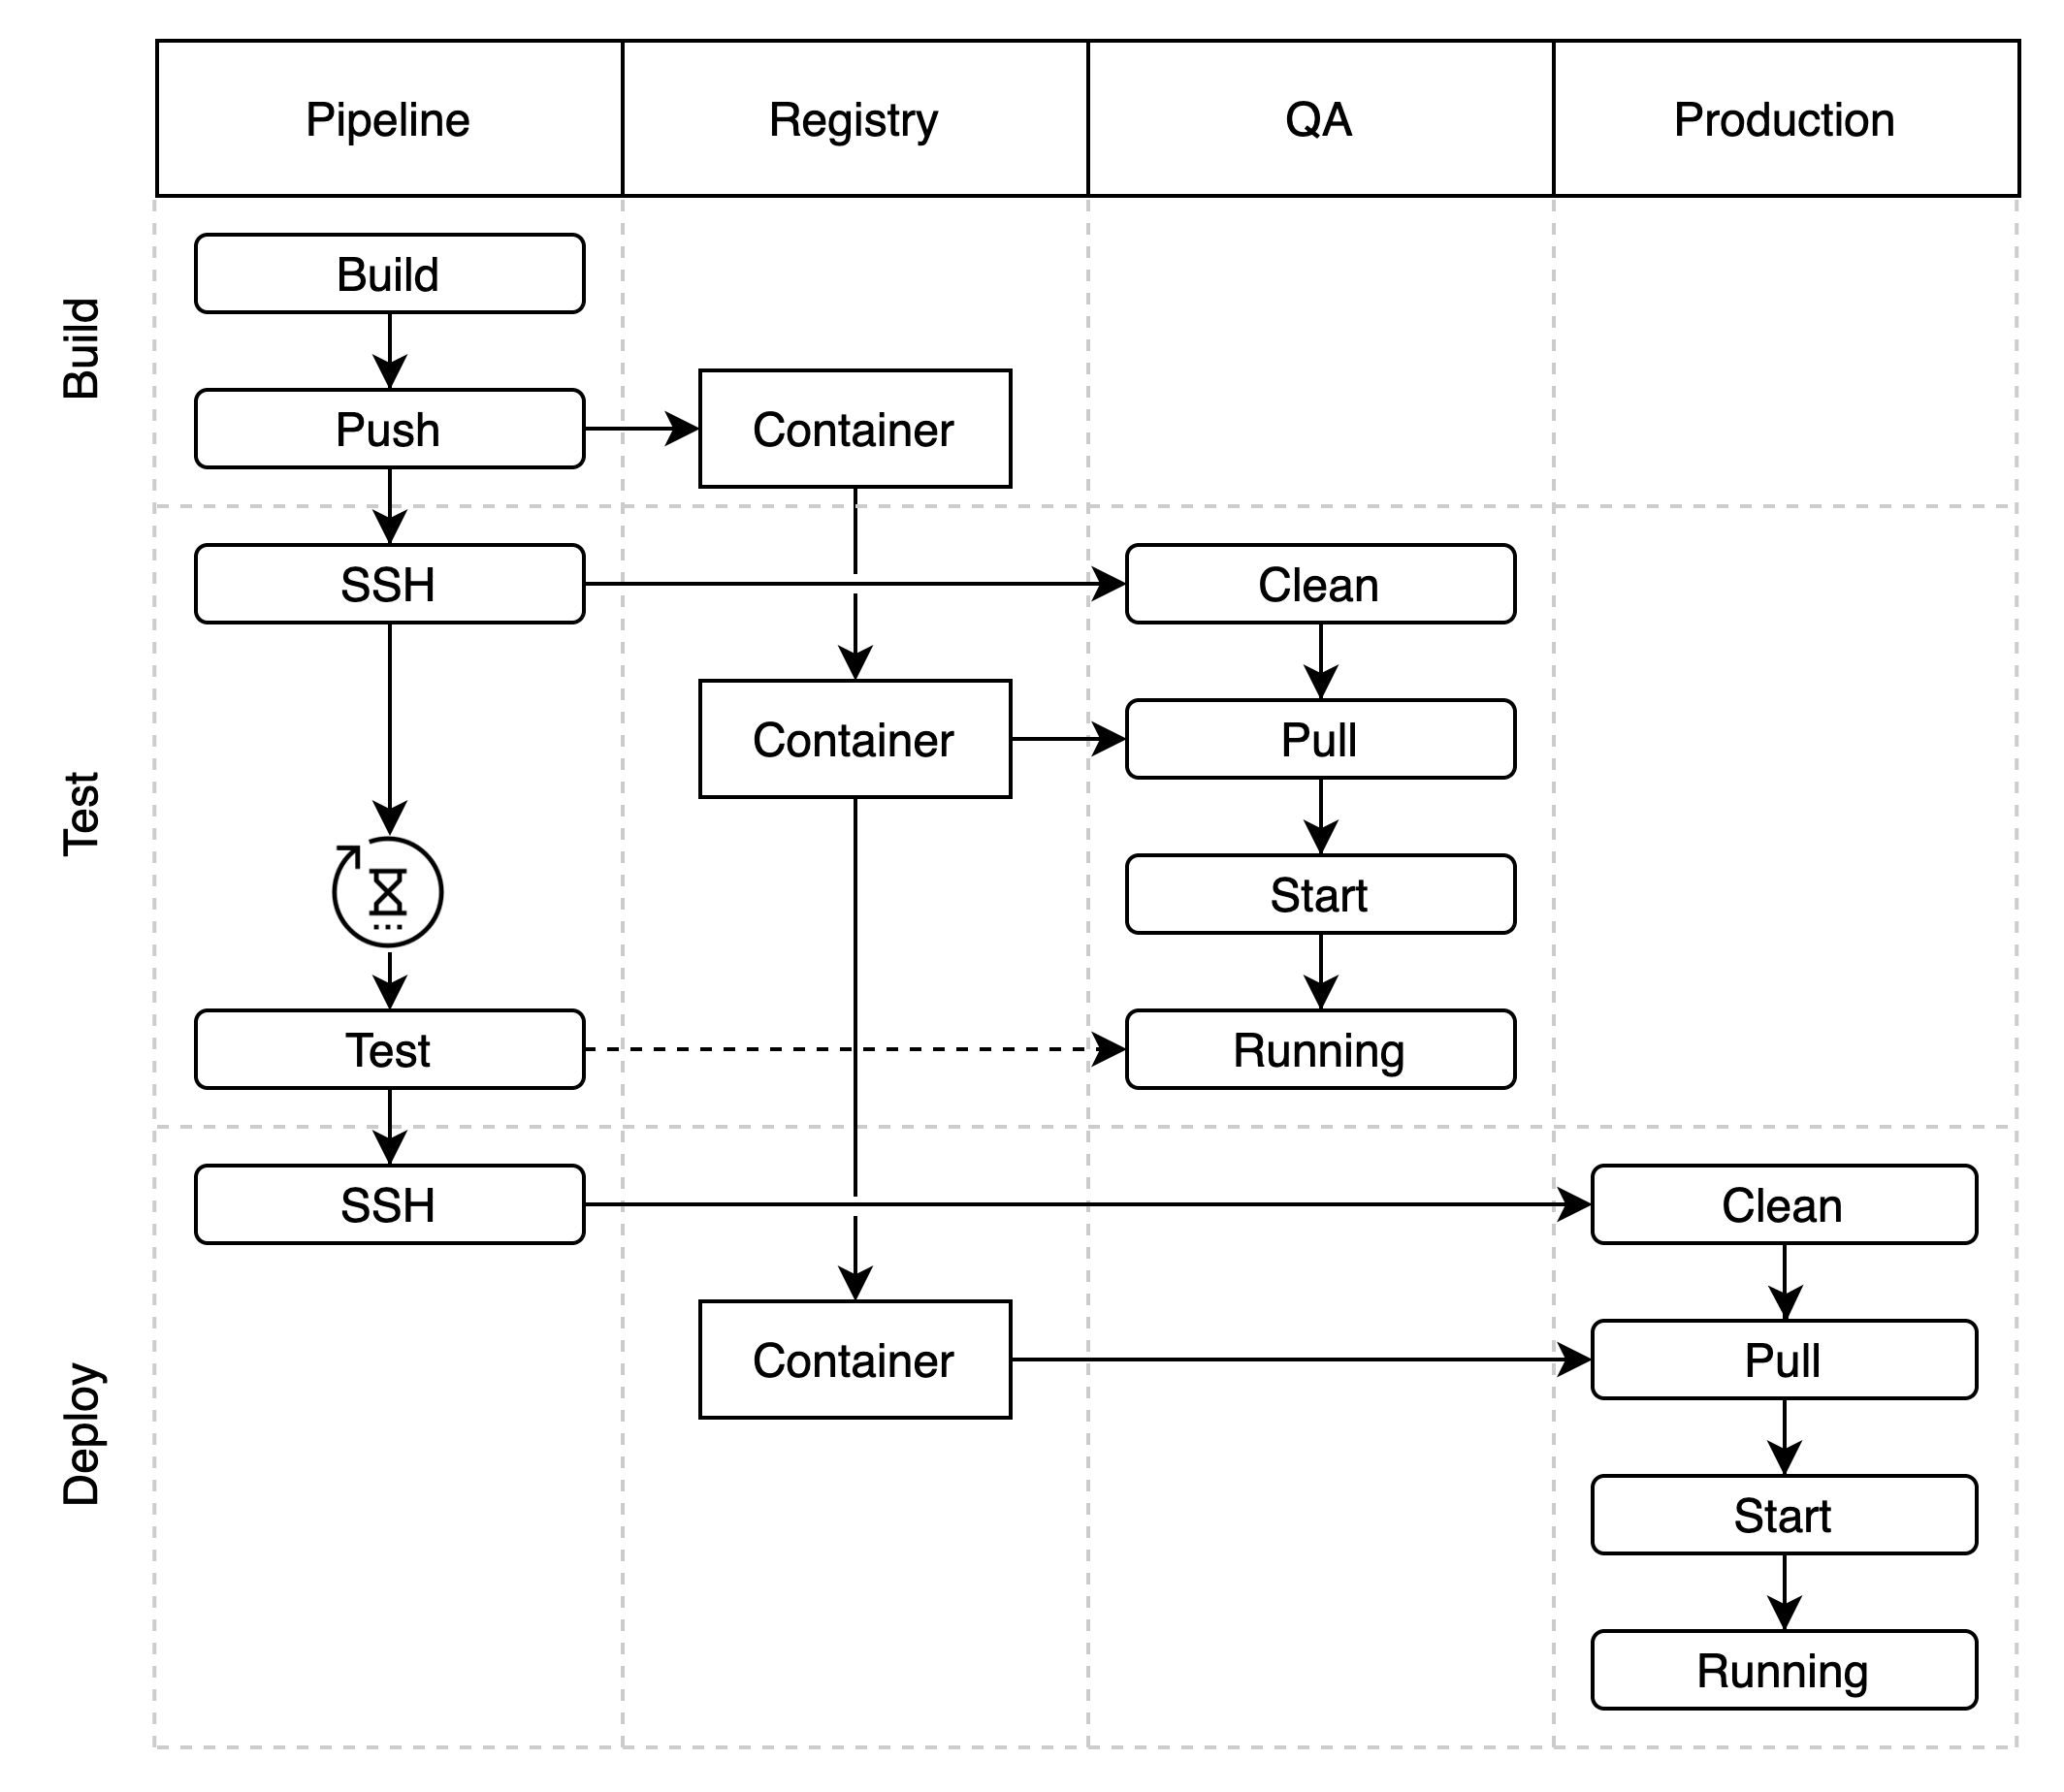
\includegraphics[scale=0.2]{img/abbildungen/Pipeline}
    \end{center}
    \caption{Übersicht über den stetigen Auslieferungsprozess}
    \label{figure:uebersichtueberdenstetigenauslieferungsprozess}
\end{figure}

An zweiter Stelle
befindet sich die Docker Registry. Eine Docker Registry ist für die Umgebung
einer Softwareanwendung das, was eine Git Repository für den Quellcode ist.
Eine Docker Registry ist also eine Art Versionsverwaltung für Docker-Images.
Hat man die Images einmal getestet, kann man davon ausgehen, dass es sich
in ausgeliefertem Zustand genauso verhalten wird, wie dies beim Testen der Fall war.

An dritter Stelle kommt die die Umgebung für die Qualitätssicherung.\footnote{Auf English Quality Assurance, abgekürzt QA.}
Hier wird die Software nach ihrer Qualität getestet. Erst wenn sie eine
zuvor definierte Qualitätsmerkmale aufweißt, darf diese in die Produktionsumgebung
ausgeliefert werden. Nach dem Buch Software-Qualität von Peter Liggesmeyer
ist ein Qualitätsmerkmal, eine "Eigenschaft einer Funktionseinheit, anhand derer ihre \(\rightarrow\)
Qualität beschrieben und beurteilt wird, die jedoch keine Aussage über
den Grad der Ausprägung enthält. Ein Qualitätsmerkmal kann über mehrere Stufen in Teilmerkmale
verfeinert werden."\cite[S. 515]{SoftwareQualitaet} Typische Qualitätsmerkmale in der Softwareentwicklung
sind Korrektheit, Vollständigkeit, Sicherheit, Zuverlässigkeit, Verfügbarkeit und Robustheit.\cite[S. 5]{SoftwareQualitaet}
Die QA bietet sich besonders gut für Integrations- sowie End-to-End-Tests an. Diese testen
das Zusammenspiel der einzelnen Komponenten. Mehr zu den einzelnen Testarten und derer Implementation
ist in \Cref{chap:qualitaetssicherung} beschrieben.

An letzter Stelle kommt die Produktionsumgebung. Hier werden die laufenden Container durch
die neuen Container, welche alle Tests erfolgreich absolviert haben, ersetzt. Die Produktionsumgebung
unterscheidet sich von der QA-Umgebung daran, dass hier die einzelnen Container je nach Verarbeitungsmenge
skaliert werden.

Als nächstes werden in \Cref{subsec:stages} die einzelnen Stages, also die Abschnitte der Pipeline
beschrieben. Daraufhin geht die Arbeit in \Cref{subsec:dockercomposesetup} auf den Aufbau von Docker-Compose ein.
In \Cref{subsec:umgebungsvariablen} wird beschrieben, wie die Arbeit mit den Umgebungsvariablen umgeht.
Zuallerletzt wird in \Cref{subsec:healthcheck} das Konzept der Health-Checks beschrieben.

\subsection{Stages}
\label{subsec:stages}
In Abbildung \ref{figure:uebersichtueberdenstetigenauslieferungsprozess} des vorherigen Abschnitts
sieht man auf der Y-Achse die Stages, die die Pipeline bei dem Auslieferungsprozess durchläuft.
Genauso wie das System der eigentlichen Anwendung besteht auch die Pipeline aus unterschiedlichen
Docker-Containern. Somit ist jeder der Abschnitte unabhängig von dem Gesamtgeschehen der Pipeline.
Öfter auftretende Funktionalitäten können in der Gitlab-CI-Pipeline in eigene Scripts ausgelagert
werden. So verhindert man redundanten Quellcode in der Pipeline. Ein Beispiel hierfür
ist Quellcode \ref{lst:wiederverwendbarescriptsdergitlabci}. Das erste ausgelagerte
Script ermöglicht das verwenden von SSH innerhalb der Pipeline. Somit kann sich
die pipeline mit dem Server verbinden, um die Docker-Compose Datei auf den Server
zu kopieren und diese auszuführen. Das zweite Script ist dafür zuständig,
sich in die Docker Registry einzuloggen. Dies ist nötig, um Docker-Container
in die Registry zu speichern und diese später vom Server aus wieder abzufragen.

\begin{listing}
    \inputminted{yaml}{snippets/yml/reusable_scripts.yml}
    \caption{Wiederverwendbare Scripts der Gitlab-CI}
    \label{lst:wiederverwendbarescriptsdergitlabci}
\end{listing}

Für die Build- und Deploy-Stage wird ein von Docker vorgefertigtes Git-Image verwendet.
Die Test-Stage verwendet ein vorgefertigtes Node.js Image mit der Version 12. Dies ist notwendig,
um die Integrationstests auszuführen, welche in JavaScript geschrieben sind.

\subsection{Docker-Compose Setup}
\label{subsec:dockercomposesetup}

\subsection{Umgebungsvariablen}
\label{subsec:umgebungsvariablen}




\subsection{Health-Checks}
\label{subsec:healthcheck}
In Microservice-Infrastrukturen sind die einzelnen Services eng miteinander verknüpft
und voneinander abhängig. Um die Verfügbarkeit sicherzustellen, werden auf
Serviceebene Healthcheckendpunkte bereitgestellt. Diese spiegeln den aktuellen
Gesundheitszustand des jeweiligen Dienstes wieder. Ein Healthcheckendpunkt
ist speziell dann nützlich, wenn ein Dienst oder ein Verfahren von einem anderen
abhängig ist. So ist beispielsweise die Backendapi von der Datenbank
abhängig. Andererseits ist der Frontenddienst sowie das Apitestverfahren
in der Buildpipeline von der Backendapi abhängig. 

\begin{listing}
    \label{lst:healthcheck}
    \inputminted{sh}{snippets/sh/healthcheck.sh}
    \caption{Healthcheckbeispiel in der Gitlab CI}
\end{listing}

\section{Web App}
\subsection{Die Zentrierung service-relevanter Einstellungen}
% extraction von theme colors etc.

\subsection{Zwischenspeicherstrategie im Service Worker}
Ein Service Worker ist ein in JavaScript geschriebener,
eventbasierter Proxy, welcher in einem separaten Thread im Browser
läuft und an eine spezifische Origin gekoppelt ist. Er hat
die Möglichkeit Anfragen zwischen der im Browser ausgeführten
Anwendung und dem Server abzufangen und zu verarbeiten.

Cache Only
Network Only
Cache First
Network First
Cache then Network
Stale while Revalidate
Generic Fallback

\begin{description}
    \item[Für den Zwischenspeicher des Browsers relevante Untergliederung]~\par
    \begin{itemize}
       \item Statische Dateien mit Hash
       \begin{itemize}
            \item main.dd5a1ad0.chunk.css
            \item main.46e36a4b.chunk.js
            \item 2.dc039c03.chunk.js
       \end{itemize}
       \item Statische Dateien ohne Hash
       \begin{itemize}
            \item index.html
            \item manifest.json
            \item favicon.ico
       \end{itemize}
       \item JSON Ressourcen von AJAX Anfragen
    \end{itemize}
\end{description}

Daraus folgende Zwischenspeicherstrategien:

\begin{description}
    \item[Zwischenspeicherstrategie]~\par
    \begin{enumerate}
       \item Statische Dateien mit Hash
       \begin{enumerate}
          \item Zuerst aus dem Zwischenspeicher anfragen
          \item Falls nicht vorhanden, aus dem Netzwerk laden und in den Zwischenspeicher ablegen
       \end{enumerate}
       \item Statische Dateien ohne Hash
       \begin{enumerate}
            \item Zuerst aus dem Netzwerk anfragen und in den Zwischenspeicher ablegen
            \item Falls keine Netzwerkverbindung vorhanden, aus dem Zwischenspeicher laden
        \end{enumerate}
        \item JSON Ressourcen von AJAX Anfragen
        \begin{enumerate}
             \item Zuerst aus dem Netzwerk anfragen
             \item Falls nicht vorhanden, Offline-Rückfallseite anzeigen 
         \end{enumerate}
    \end{enumerate}
 \end{description}

 % Probleme: Plugin Bundle Quellcode und Markdown seiten


\subsection{Healthcheck}
% logout in one browser tab

\subsection{Seitengenerator}
% die verschiedenen Seiten sollten für das caching evtl. mit einem hash on build time versehen werden.

\subsection{Sprachauswahl}

\subsection{Modaldesign}

\subsection{Stetige Aktualisierung der PWA}
Probleme: cookies verändern sich, Service Worker verändert sich, neue Felder in der Datenbank
Frontend und Backend etc, also allen verschiedenen Services

\section{Benutzerverwaltung}
\subsection{Mailserver}
\subsection{Two-factor Auth}
\subsection{Two-Way Validation}
\subsection{Die Rechteverwaltung}
\subsection{One verification route}
\subsection{Horizontale Skalierung ermöglichen}
% stateless backend, no sessions etc.


\section{Datenlieferung}

\begin{figure}
    \label{figure:informationsaustauschdashboard}
    \begin{center}
    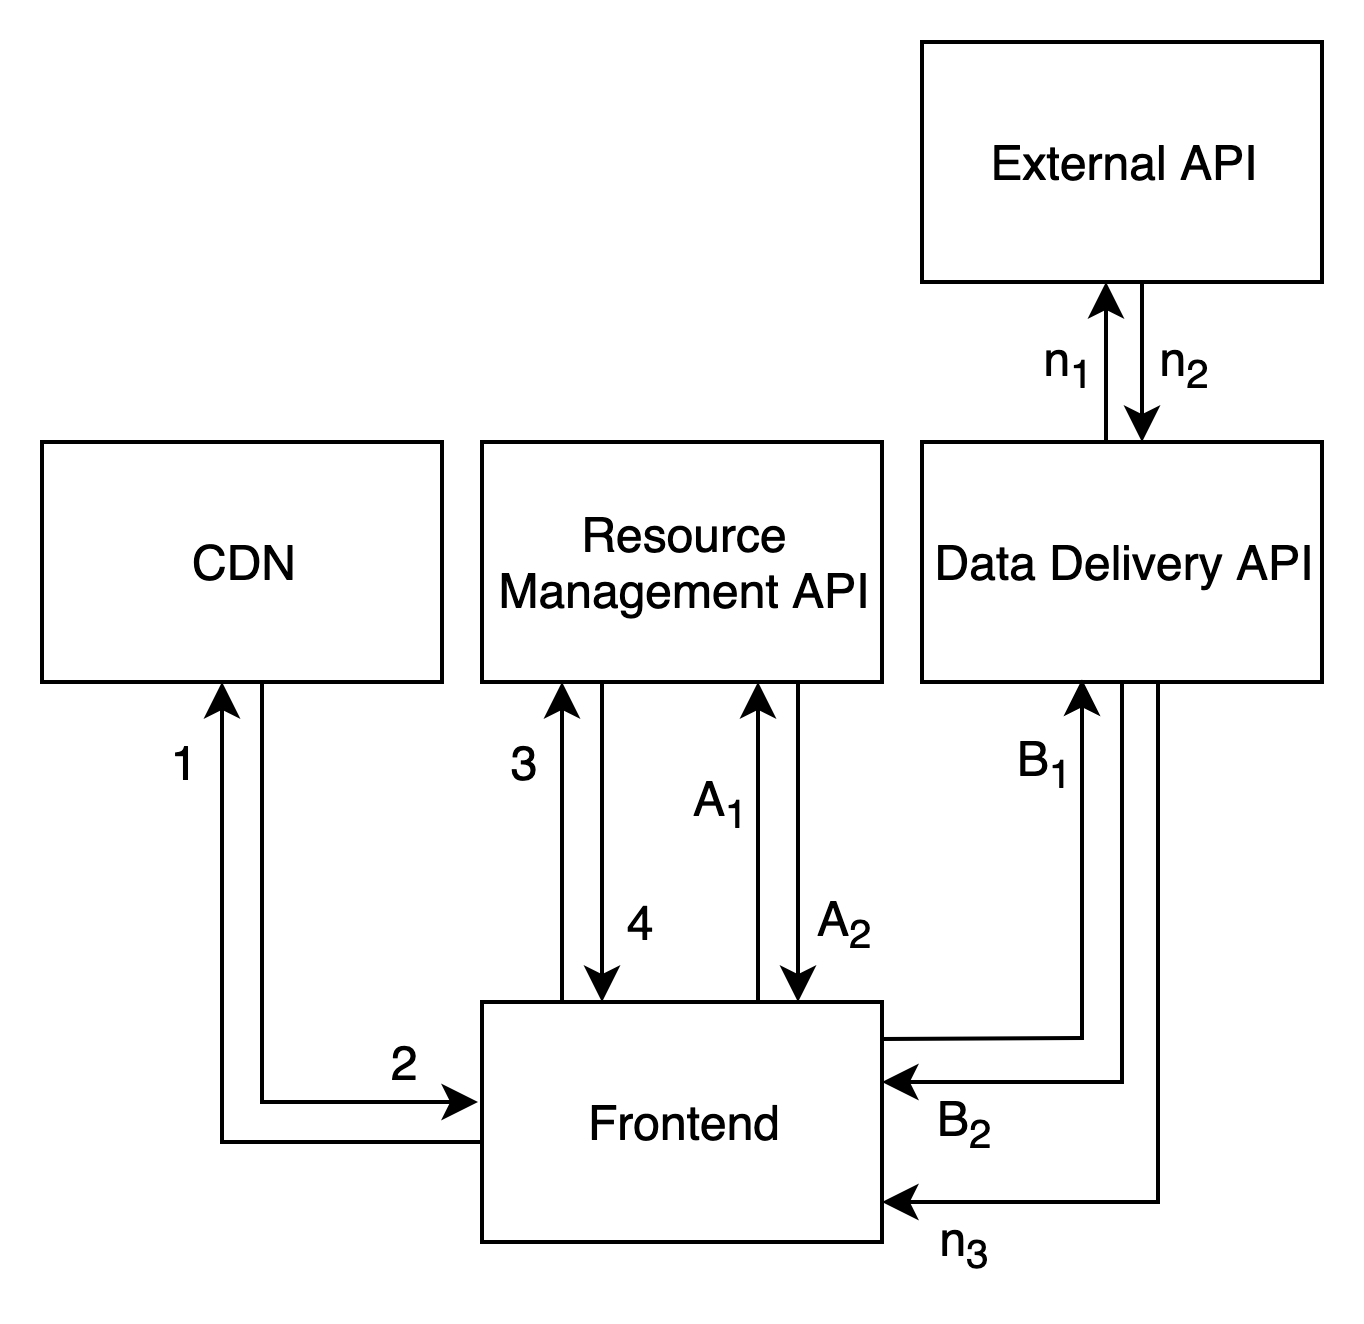
\includegraphics[scale=0.2]{img/abbildungen/InformationsaustauschDashboard}
    \end{center}
    \caption{Ablauf des Informationsaustausches eines Dashboards}
\end{figure}

\begin{figure}
    \label{figure:uebersichtderdatenauslieferung}
    \begin{center}
    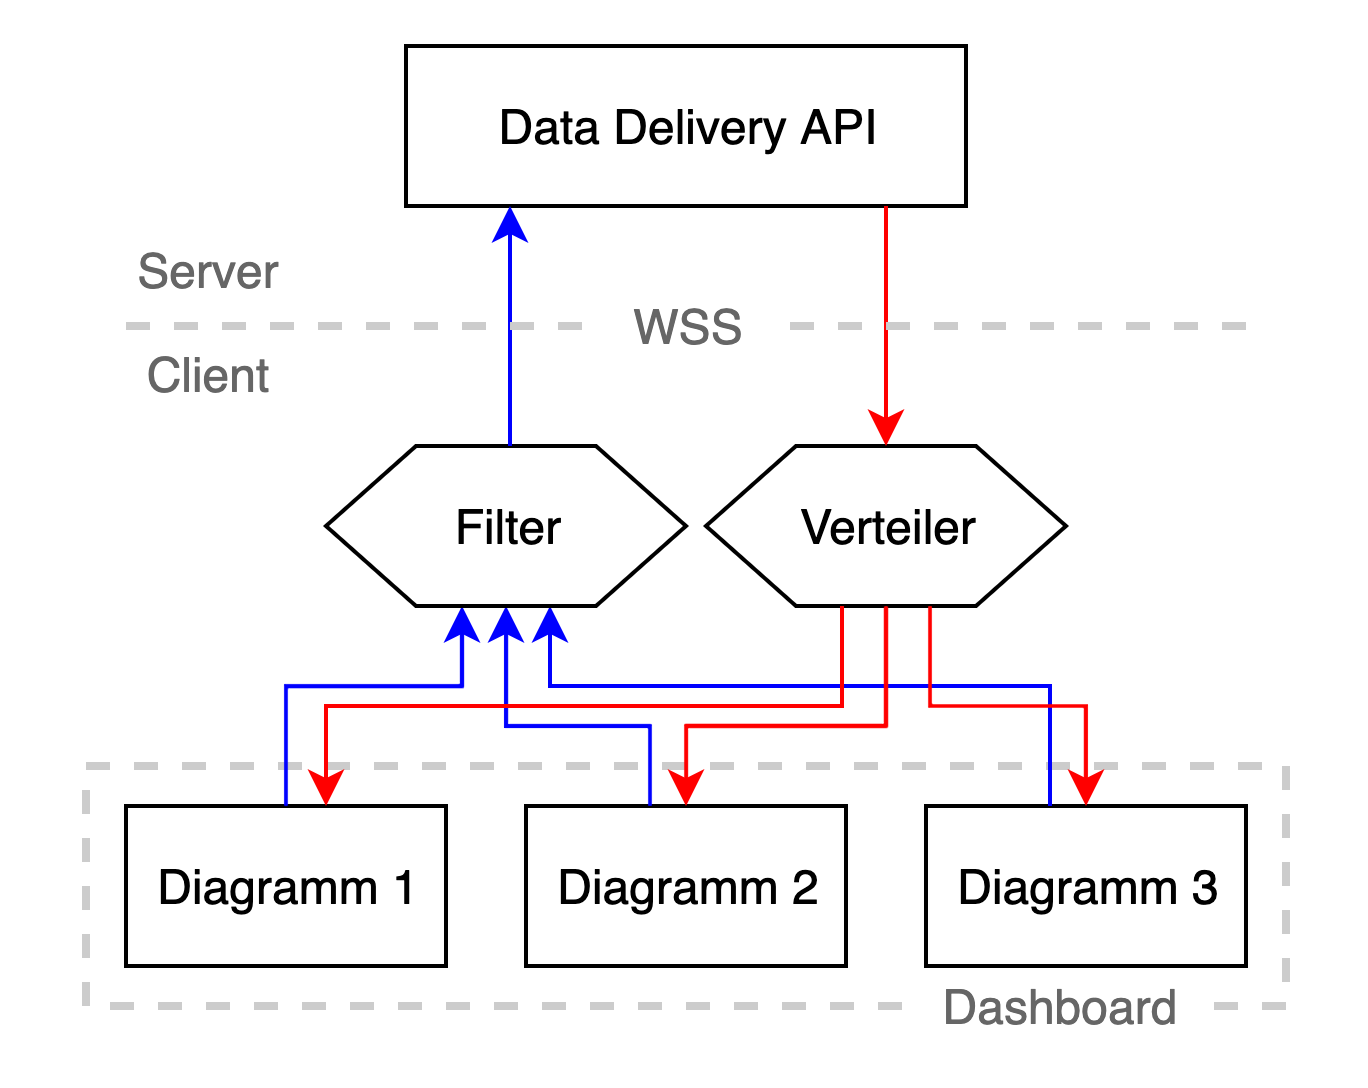
\includegraphics[scale=0.2]{img/abbildungen/Verteilung}
    \end{center}
    \caption{Verringerung der Redundanz des Datenflusses}
\end{figure}

\begin{figure}
    \label{figure:screenshotdeswebsocketdatenverkehrs}
    \begin{center}
    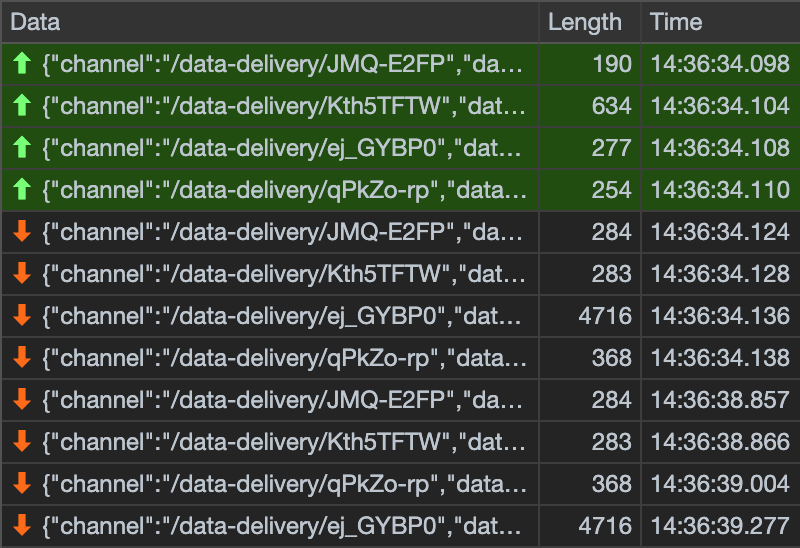
\includegraphics[scale=0.65]{img/screenshots/WebSocketTraffic}
    \end{center}
    \caption{Screenshot des WebSocket-Datenverkehrs}
\end{figure}
% Erkenntnis, Der Cache ist viel schneller, Cache ist O(1) wohingegen datenverarbeitung O(n) ist siehe
% anhand der größeren Anfrage

\subsection{WWS Handshake Authentifizierung}
\subsection{Golang MongoDB Aufbau}

\section{Plugins}
\subsection{Code Splitting und Lazy Loading}
% loading plugins on runtime
\subsection{D3.js und Chart.js}
\begin{listing}
    \label{lst:HelloJSX}
    \caption{Ein einfaches JSX Beispiel}
    \inputminted{jsx}{snippets/examples/Welcome.jsx}
\end{listing}

\begin{listing}
    \label{lst:Golang}
    \caption{Ein einfaches Golang Beispiel}
    \inputminted{go}{snippets/examples/hello.go}
\end{listing}
